\section{Model analysis}

\subsection{Question types}

Model performance on SQuAD 2.0 can be categorized based on whether the question-context pair has an answer (Has Answer versus No Answer). The dev set is very balanced in this sense as it contains 5,928 ($\sim$49.93\%) pairs with answers and 5,945 ($\sim$50.07\%) pairs without answers. Figure [\ref{fig:qa_correct_answers_by_model_and_type}] shows the fraction of questions of each type that BERT and our best-performing models correctly answers. As BERT is fine-tuned, the number of correctly answered questions in both categories increases, but questions with “No Answer” increases more rapidly. Our best models answer more “No Answer” questions correctly than BERT, but underperform BERT in terms of “Has Answer” questions.

To investigate further, we looked at our 3/10 epoch model’s incorrect predictions on “Has Answer” questions, and found that a large percentage, $\sim$65\%, were predicted as having no answer (rather than with the wrong answer). These results suggest that our models may be more liberal than BERT at predicting “no answer.”

\begin{figure}[ht]
	\centering
	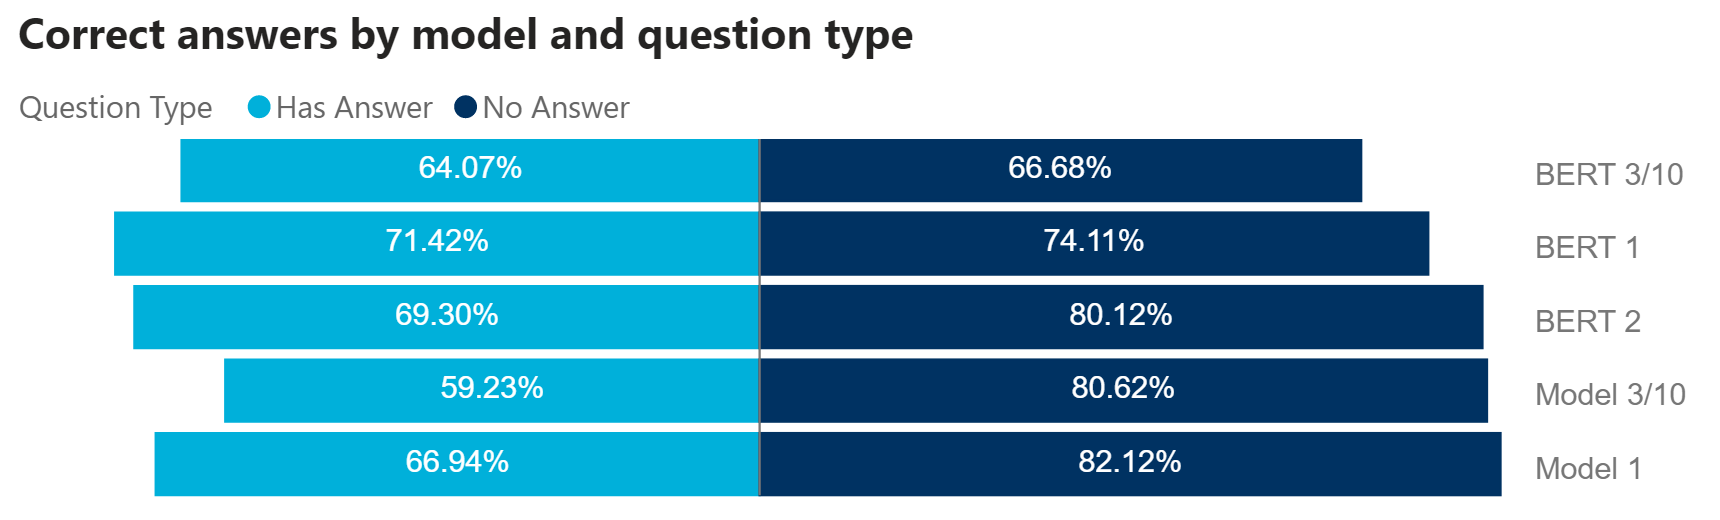
\includegraphics[width=7.5cm]{images/QA_Correct_Answers_by_Question_Type.png}
	\caption{\label{fig:qa_correct_answers_by_model_and_type}Correctly answered percentages by model}
\end{figure}

\subsection{Second most likely answer}

For questions where our 3/10 epoch model’s most likely answer was incorrect, we considered the second most likely answer predicted by the model. We found that the second most likely answer is correct 44\% of the time when the most likely answer is incorrect. We also note 47\% of these were also “Has Answer” questions, which is a more balanced distribution compared to the most likely answer (where only 42\% of correctly answered questions have an answer). This suggests that even though our model at 3/10 is liberal at predicting no answer, its second most likely answer is quite frequently correct and less biased. 

\subsection{Context Length}

The previous section shows that our models are better at recognizing questions with no answers compared to BERT. Here, we look at which models perform better on longer sequences. At 3/10 of an epoch of fine-tuning, BERT and our models performed similarly (BERT average length: 165.86, our model average length: 164.50). However, we believe this is because both models answered many of the same questions correctly. When looking at questions that were uniquely answered correctly by each model, a clear difference emerges: the average sequence length for BERT is longer (BERT: 175.30, our model: 161.58). This suggests that our models are better at answering questions with shorter contexts than BERT. The same trend holds at 1 epoch of fine-tuning.

\subsection{Do 2 epochs perform even better?}
	
Our previous results show that models built on BERT embeddings at 1 epoch achieves maximal BERT performance at 2 epochs. Here, we investigate if we can further improve performance by training directly on embeddings derived at 2 epochs. While this approach does not reduce BERT fine-tuning time, it does provide a way to investigate whether our approach can achieve even better performance with longer fine-tuning. 
	
Table [\ref{tbl:bc_bert_fine_tuning}] shows the results. As expected, the 2-epoch models outperform the same models trained on 1-epoch embeddings. Since ensembling improved performance at 1 epoch, we applied the same approach to the models at 2 epochs. Surprisingly, the 2 epoch ensemble does not outperform the 1 epoch ensemble in terms of either EM (0.749 vs 0.756) or F1 (0.795 vs 0.798). This suggests that additional fine-tuning does not guarantee better performance. Our 1-epoch models, in addition with ensembling, not only saves on BERT fine-tuning time, but also achieves the best possible performance, suggesting a total lack of need for fine-tuning beyond 1 epoch.

\begin{table}[ht]
	\centering
	\small
	\begin{tabular}{L{4.2cm}|C{0.9cm} C{0.9cm}}
		\toprule
		\textbf{Model} & \multicolumn{2}{c}{\textbf{SQuAD2.0}}\\
		& \textbf{EM} & \textbf{F1}\\
		\midrule
		BERT $2e$ (\textit{best}) 		& $0.747$ & $0.792$ \\
		best model architecture from $1e$	& $0.753$ & $0.797$ \\
		best model architecture from $\frac{3}{10}e$ 		& $0.749$ & $0.795$ \\
		ensemble BERT $2e$ + best $1e$	& $0.751$ & $0.796$ \\
		\bottomrule
	\end{tabular}
	\caption{\label{tbl:bc_bert_fine_tuning}Models trained on embeddings at 2 epochs}
\end{table}
